\documentclass[tikz,border=2pt]{standalone}
\usepackage{amsmath,amssymb}
\usepackage{tikz}
\usetikzlibrary{arrows.meta,calc}

\begin{document}
% Among all unit directions u at a, the directional derivative grad f(a) . u is largest for u
% pointing along the gradient (perpendicular to the level set), zero along the level set,
% and most negative opposite to the gradient.
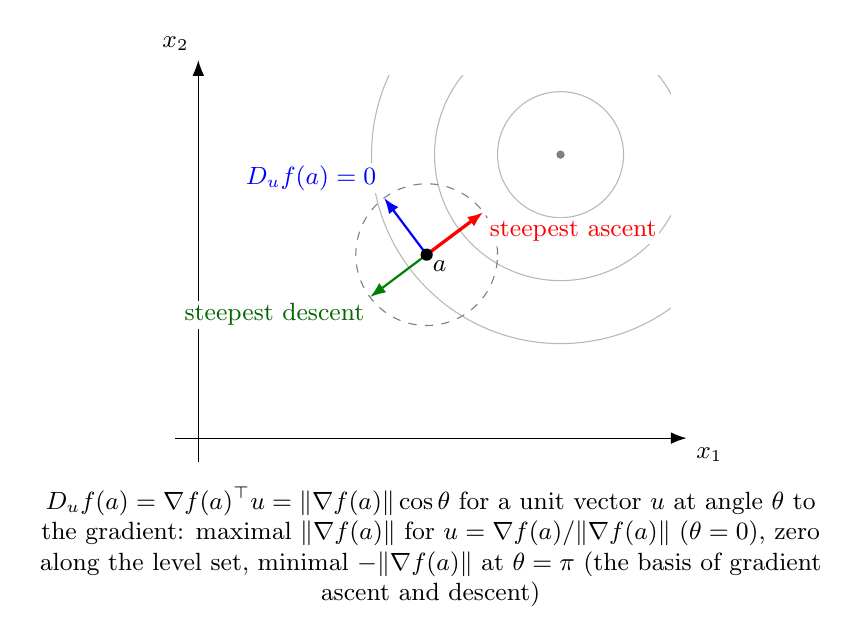
\begin{tikzpicture}[every node/.style={font=\small}, >={Latex[length=2mm]}, lab/.style={font=\small, fill=white, inner sep=1pt}]
	\begin{scope}
		\clip (0,0) rectangle (6.0,4.6);
		\foreach \r in {0.8,1.6,2.4} {\draw[gray!55] (4.6,3.6) circle (\r);}
	\end{scope}
	\fill[gray] (4.6,3.6) circle (1.5pt);
	\draw[->] (-0.3,0) -- (6.2,0) node[below right] {$x_1$};
	\draw[->] (0,-0.3) -- (0,4.8) node[above left] {$x_2$};
	\coordinate (A) at (2.9,2.33);
	\draw[gray, dashed] (A) circle (0.9);
	\draw[->, red, very thick] (A) -- ($(A)+(0.72,0.54)$);
	\node[red, lab, anchor=north west] at (3.66,2.8) {steepest ascent};
	\draw[->, blue, thick] (A) -- ($(A)+(-0.54,0.72)$);
	\node[blue, lab, anchor=south east] at (2.3,3.1) {$D_uf(a)=0$};
	\draw[->, green!50!black, thick] (A) -- ($(A)+(-0.72,-0.54)$);
	\node[green!40!black, lab, anchor=north east] at (2.15,1.75) {steepest descent};
	\fill (A) circle (2.2pt) node[below right, inner sep=2pt] {$a$};
	\node[anchor=north, align=flush center, text width=10cm] at (2.95,-0.5) {$D_uf(a)=\nabla f(a)^{\top}u=\|\nabla f(a)\|\cos\theta$ for a unit vector $u$ at angle $\theta$ to the gradient: maximal $\|\nabla f(a)\|$ for $u=\nabla f(a)/\|\nabla f(a)\|$ ($\theta=0$), zero along the level set, minimal $-\|\nabla f(a)\|$ at $\theta=\pi$ (the basis of gradient ascent and descent)};
\end{tikzpicture}
\end{document}
